% Options for packages loaded elsewhere
\PassOptionsToPackage{unicode}{hyperref}
\PassOptionsToPackage{hyphens}{url}
%
\documentclass[
]{article}
\usepackage{amsmath,amssymb}
\usepackage{iftex}
\ifPDFTeX
  \usepackage[T1]{fontenc}
  \usepackage[utf8]{inputenc}
  \usepackage{textcomp} % provide euro and other symbols
\else % if luatex or xetex
  \usepackage{unicode-math} % this also loads fontspec
  \defaultfontfeatures{Scale=MatchLowercase}
  \defaultfontfeatures[\rmfamily]{Ligatures=TeX,Scale=1}
\fi
\usepackage{lmodern}
\ifPDFTeX\else
  % xetex/luatex font selection
\fi
% Use upquote if available, for straight quotes in verbatim environments
\IfFileExists{upquote.sty}{\usepackage{upquote}}{}
\IfFileExists{microtype.sty}{% use microtype if available
  \usepackage[]{microtype}
  \UseMicrotypeSet[protrusion]{basicmath} % disable protrusion for tt fonts
}{}
\makeatletter
\@ifundefined{KOMAClassName}{% if non-KOMA class
  \IfFileExists{parskip.sty}{%
    \usepackage{parskip}
  }{% else
    \setlength{\parindent}{0pt}
    \setlength{\parskip}{6pt plus 2pt minus 1pt}}
}{% if KOMA class
  \KOMAoptions{parskip=half}}
\makeatother
\usepackage{xcolor}
\usepackage[margin=1in]{geometry}
\usepackage{color}
\usepackage{fancyvrb}
\newcommand{\VerbBar}{|}
\newcommand{\VERB}{\Verb[commandchars=\\\{\}]}
\DefineVerbatimEnvironment{Highlighting}{Verbatim}{commandchars=\\\{\}}
% Add ',fontsize=\small' for more characters per line
\usepackage{framed}
\definecolor{shadecolor}{RGB}{248,248,248}
\newenvironment{Shaded}{\begin{snugshade}}{\end{snugshade}}
\newcommand{\AlertTok}[1]{\textcolor[rgb]{0.94,0.16,0.16}{#1}}
\newcommand{\AnnotationTok}[1]{\textcolor[rgb]{0.56,0.35,0.01}{\textbf{\textit{#1}}}}
\newcommand{\AttributeTok}[1]{\textcolor[rgb]{0.13,0.29,0.53}{#1}}
\newcommand{\BaseNTok}[1]{\textcolor[rgb]{0.00,0.00,0.81}{#1}}
\newcommand{\BuiltInTok}[1]{#1}
\newcommand{\CharTok}[1]{\textcolor[rgb]{0.31,0.60,0.02}{#1}}
\newcommand{\CommentTok}[1]{\textcolor[rgb]{0.56,0.35,0.01}{\textit{#1}}}
\newcommand{\CommentVarTok}[1]{\textcolor[rgb]{0.56,0.35,0.01}{\textbf{\textit{#1}}}}
\newcommand{\ConstantTok}[1]{\textcolor[rgb]{0.56,0.35,0.01}{#1}}
\newcommand{\ControlFlowTok}[1]{\textcolor[rgb]{0.13,0.29,0.53}{\textbf{#1}}}
\newcommand{\DataTypeTok}[1]{\textcolor[rgb]{0.13,0.29,0.53}{#1}}
\newcommand{\DecValTok}[1]{\textcolor[rgb]{0.00,0.00,0.81}{#1}}
\newcommand{\DocumentationTok}[1]{\textcolor[rgb]{0.56,0.35,0.01}{\textbf{\textit{#1}}}}
\newcommand{\ErrorTok}[1]{\textcolor[rgb]{0.64,0.00,0.00}{\textbf{#1}}}
\newcommand{\ExtensionTok}[1]{#1}
\newcommand{\FloatTok}[1]{\textcolor[rgb]{0.00,0.00,0.81}{#1}}
\newcommand{\FunctionTok}[1]{\textcolor[rgb]{0.13,0.29,0.53}{\textbf{#1}}}
\newcommand{\ImportTok}[1]{#1}
\newcommand{\InformationTok}[1]{\textcolor[rgb]{0.56,0.35,0.01}{\textbf{\textit{#1}}}}
\newcommand{\KeywordTok}[1]{\textcolor[rgb]{0.13,0.29,0.53}{\textbf{#1}}}
\newcommand{\NormalTok}[1]{#1}
\newcommand{\OperatorTok}[1]{\textcolor[rgb]{0.81,0.36,0.00}{\textbf{#1}}}
\newcommand{\OtherTok}[1]{\textcolor[rgb]{0.56,0.35,0.01}{#1}}
\newcommand{\PreprocessorTok}[1]{\textcolor[rgb]{0.56,0.35,0.01}{\textit{#1}}}
\newcommand{\RegionMarkerTok}[1]{#1}
\newcommand{\SpecialCharTok}[1]{\textcolor[rgb]{0.81,0.36,0.00}{\textbf{#1}}}
\newcommand{\SpecialStringTok}[1]{\textcolor[rgb]{0.31,0.60,0.02}{#1}}
\newcommand{\StringTok}[1]{\textcolor[rgb]{0.31,0.60,0.02}{#1}}
\newcommand{\VariableTok}[1]{\textcolor[rgb]{0.00,0.00,0.00}{#1}}
\newcommand{\VerbatimStringTok}[1]{\textcolor[rgb]{0.31,0.60,0.02}{#1}}
\newcommand{\WarningTok}[1]{\textcolor[rgb]{0.56,0.35,0.01}{\textbf{\textit{#1}}}}
\usepackage{longtable,booktabs,array}
\usepackage{calc} % for calculating minipage widths
% Correct order of tables after \paragraph or \subparagraph
\usepackage{etoolbox}
\makeatletter
\patchcmd\longtable{\par}{\if@noskipsec\mbox{}\fi\par}{}{}
\makeatother
% Allow footnotes in longtable head/foot
\IfFileExists{footnotehyper.sty}{\usepackage{footnotehyper}}{\usepackage{footnote}}
\makesavenoteenv{longtable}
\usepackage{graphicx}
\makeatletter
\def\maxwidth{\ifdim\Gin@nat@width>\linewidth\linewidth\else\Gin@nat@width\fi}
\def\maxheight{\ifdim\Gin@nat@height>\textheight\textheight\else\Gin@nat@height\fi}
\makeatother
% Scale images if necessary, so that they will not overflow the page
% margins by default, and it is still possible to overwrite the defaults
% using explicit options in \includegraphics[width, height, ...]{}
\setkeys{Gin}{width=\maxwidth,height=\maxheight,keepaspectratio}
% Set default figure placement to htbp
\makeatletter
\def\fps@figure{htbp}
\makeatother
\setlength{\emergencystretch}{3em} % prevent overfull lines
\providecommand{\tightlist}{%
  \setlength{\itemsep}{0pt}\setlength{\parskip}{0pt}}
\setcounter{secnumdepth}{-\maxdimen} % remove section numbering
\ifLuaTeX
  \usepackage{selnolig}  % disable illegal ligatures
\fi
\usepackage{bookmark}
\IfFileExists{xurl.sty}{\usepackage{xurl}}{} % add URL line breaks if available
\urlstyle{same}
\hypersetup{
  pdftitle={Seasonal patterns on isotopic niches and diet of Bigeye and Southern Spotted Opah (Lamprididae) in Southwestern Atlantic Ocean},
  hidelinks,
  pdfcreator={LaTeX via pandoc}}

\title{Seasonal patterns on isotopic niches and diet of Bigeye and
Southern Spotted Opah (Lamprididae) in Southwestern Atlantic Ocean}
\author{true \and true \and true}
\date{}

\begin{document}
\maketitle

abstract: \textbar{} Opahs (Lampsis spp.) are large deep-water
epi-mesopelagic predator fishes captured worldwide as bycatch of
longline fisheries targeting large pelagic fishes. Despite the growing
culinary interest leading to increasing commercial interest, several
basic biological information about the species is still poorly known.
This study uses stable isotope and stomach content analysis to access
the diet and seasonality on the isotopic niche of the Big-eye Opah,
Lampris megalopsis, and the Southern Spotted Opah Lampris australensis
in the Southwest Atlantic Ocean (SWAO). Generalized Linear Models were
applied to investigate the influence of the species, sex, seasons, and
furcal length on 13C and 15N isotopic compositions. Significant
differences were observed only for Autumn and for L. megalopsis. The
isotopic niches resulted in overlapped 40\% ellipses between the
species. Seasonal differences for 15N in hot and cold seasons for both
species related to the dynamic of the Brazilian and the Malvinas
(Falkland) currents and the shift on the baseline source of nitrogen.
Differences in 13C, with enriched values in the warmer season, were
observed only for L. megalopsis and suggested movements to areas with
depleted 15C values. Diet for both species was composed predominantly by
Cephalopods and Teleost's, followed by Crustacea, in smaller quantities.
An alarming high plastic frequency of occurrence was observed in 40\% of
the stomachs of L. megalopsis and 31\% of L. australensis. This study
advances in understanding the Opah fishes feeding ecology in SWAO and
provides information on community dynamics and the functional role that
these species play in the structure of all marine ecosystems where they
occur. Given the growing global commercial importance of Lampris spp.,
it is also increasingly important to know their inter and intraspecific
relationships and the anthropological impacts they are suffering.

keywords: - Lampris - 13C and 15N - plastic pollution

Introduction: Opahs are large deep-water epi-mesopelagic predator
fishes, generating heat with their strong pectoral fin muscles and using
it to warm their heart and brain (Wegner et al., 2015). This
characteristic increases its metabolism in cold-deep waters, which
facilitates its movements across strong thermal gradients found in the
open ocean (Polovina, 2008; Wainwright \& Longo, 2017), and making these
globally distributed fishes powerful swimmers (Rosenblatt \& Johnson,
1976; Wegner et al., 2015). Recent studies have shown that the
previously species addressed as Lampris guttatus were a complex of five
species distributed around the globe (Hyde et al., 2014; Underkoffler et
al., 2018), two of them occurring in the Southwest Atlantic Ocean
(SWAO): L. megalopsis, a cosmopolitan species, and L. australensis,
circumglobally distributed in the southern hemisphere subtropical waters
(Terlecki et al., in prep.). Only a few studies approaching the feeding
ecology of Lampris genera species have been published, including one
about the diet of L. immaculatus (Jackson et al., 2000) and four
comprising the species L. megalopsis (Big eye Opah) and L. incognitus
(Small eye Opah), about diet composition (Choy et al., 2013), trophic
level (Choy et al., 2015), plastic ingestion (Choy \& Drazen, 2013, Neto
et al., 2020) and biomass of predator fishes (Choy et al., 2016). Most
of these studies were conducted in the North Pacific Ocean and concluded
that these Opahs feed upon squids predominantly, followed by small
pelagic fishes and lesser by small octopuses and crustaceans. The
Lampris species are caught by longline fisheries around the world
targeting large pelagic fishes, such as swordfish, tunas, and sharks
(e.g., Hawn \& Collete, 2012; Huang \& Liu, 2010; Runcie, Dewar, Hawn,
Frank \& Dickson, 2009; Underkoffler, Luers, Hyde \& Craig, 2018). In
the Southwest Atlantic Ocean (SWAO), longline fishing fleets from more
than seven countries operate targeting swordfish Xiphias gladius,
pelagic sharks (mainly blue shark Prionace glauca), and several tuna
species (bigeye Thunnus obesus, yellow-fin T. albacares, and albacore T.
alalunga) throughout the year (Hazin, Broadhurst, Amorim, Arfelli \&
Domingo, 2008; Jiménez, Domingo, Abreu \& Brazeiro, 2011; Tuck,
Polacheck, \& Bulman, 2003) and, at least, two Opah species L.
megalopsis and L. australensis are incidentally caught (Terlecki et al.,
in prep.). Although, little is known about the scale of the Opahs
catches in the region. Two years of longline landings monitoring of just
the Brazilian fishing fleets operating in the region recorded 3.6 tons
in 2018 and 4.8 tons in 2019 (UNIVALI/EMCT/LEMA, 2020). Nevertheless,
despite the increasing commercial interest in its capture due to the
growing culinary interest in the quality of its meat (Underkoffler et
al., 2014), their biology is still poorly studied, and intra and
interspecific relationships are still unclear (Hyde et al., 2014, Choy
\& Drazen, 2013). The term ecological niche, described by Hutchinson
(1957), is a multidimensional space constituted by all the environmental
characteristics allowing an organism to live, thus beings a key concept
to understand how species use resources, participate in food webs, and
influence their habitat (Bearhop et al., 2004). As the feeding ecology
of species provides fundamental information on community dynamics and
the functional role that species play in the structure of ecosystems
(Braga et al., 2012), understanding trophic interactions of these
organisms contributes to revealing the functioning, structuring, and
energy flow on ecological niches (Newsome et al., 2007). Studies of fish
diet, feeding ecology, and food habits are commonly carried out by
examining gut contents (Hynes, 1950; Hyslop, 1980). However, this
technique presents some limitations, as the tendency to underestimate
prey items quickly assimilated by the consumer (Chipps and Garvey, 2007)
and to overestimate slowly digesting prey taxa or hard parts (e.g.,
cephalopod beaks), since they will tend to remain in the stomach for an
extended period (Baker et al., 2014, Hyslop, 1980). In contrast, stable
isotope analysis provides quantitative information on both resource
(bionomic) and habitat (scenopoetic) factors, commonly used to define
ecological niche space, within variable periods of time (Newsome et al.,
2007). The δ13C and δ15N values of consumers' tissues reflect those from
their prey and offset due to the metabolic processes associated with the
tissue synthesis and assimilation, often called trophic discrimination.
This generates a systematic enrichment of the heavier isotope through
the trophic levels greater for δ15N (2--4‰) than for δ13C (0--2‰)
(DeNiro and Epstein, 1978, 1981). Therefore, δ13C values are considered
adequate for estimating the influence of primary producers on the
baseline of the consumer food web (Peterson and Fry, 1987), and δ15N is
useful for trophic level estimation (Post, 2002). These premises were
the foundation to the concept of isotopic niche proposed by Newsome et
al.~(2007), which is comparable to the n-dimensional space within the
ecological niche, is composed since its preys and habitat directly
influence the isotopic animal composition. Thus, with the information
provided by δ13C and δ15N analysis, it is possible to provide
information on the scenopoetic and bionomic axes as a proxy of the
ecological niche of a species (Bearhop et al., 2004; Newsome et al.,
2007). Understanding the SWAO Opah fish feeding ecology will provide
fundamental information on community dynamics and the functional role
that this species plays in the structure of the SWAO marine ecosystem.
In this study, we assessed the seasonality on the isotopic niche of L.
megalopsis and L. australensis, and, in addition, we analyzed their
diet, recording, inclusively some plastic ingestion.

Material e Methods:

Sampling

The Opahs were collected opportunistically between july/2018 and
march/2020. Samples were taken from landings of the surface longline
fleets operating in Southwest Atlantic Ocean (SWAO) in Rio Grande, RS,
Brazil (Figure 1). The fishing region is in the western boundary of the
Subtropical Convergence (30--36◦S) formed by the confluence of the warm
and oligotrophic waters carried by the Brazilian Current and the
nutrient-rich and cold subantarctic waters of the Malvinas (Falklands)
Current (Garcia, 1997). From 88 individuals, furcal length (mm) was
measured and sixty-one muscle samples (0.5 cm³), including 42 from L.
australensis and 19 from L. megalopsis were taken for isotopic analyses.
Stomachs are commonly excised at sea. From fishes obtained at hole,
stomachs were collected and frozen at - 20°C until processing.

\begin{figure}
\centering
\includegraphics{nome-da-imagem.png}
\caption{Figura 1}
\end{figure}

Muscle samples were rinsed with distilled water washed with a methanol
and chloroform (2:1) solution in a Soxhlet reflux, for 12 hours, to
remove lipids (Bligh and Dyer, 1959). The samples were than dried in an
oven at 60 ◦C for 46 hours, ground to fine powder with mortar, and
pestle prior to analysis. Aliquots of 0.6 -- 0.7 mg of the resulting
powder were placed into tin capsules for analysis using isotope ratio
mass spectrometry (measurement precision of 0.1‰ for δ13C and 0.3‰ for
δ15N) at the Centro Integrado de Análises of the Universidade Federal do
Rio Grande (CIA-FURG, Brazil). Differences between sample rations and
the international reference standards for carbon (Vienna Pee Dee
Belenmite) and nitrogen (atmospheric air) were expressed in δ notation
as parts per thousand (‰) using the equation: \[
\delta X (‰) = \left( \frac{R_{sample}}{R_{standard}} - 1 \right) \times 1000
\] where X is 13C or 15N and R\_sample is 13C/12C or 15N/15N from the
sample and R\_standard is 13C/12C or 15N/15N from the reference standard
used (Peterson and Fry, 1987). We measured the C:N ratios of each
sample, and most of values was not in the expected range for pure
protein (Logan et al., 2008; Post, 2002). Because lipids are depleted in
13C compared with whole organisms (Peterson and Fry 1987), we expected
our samples would present a relation were as the C:N had higher values,
δ13C would present smaller ones. Although, this did not happen and, as
it was not possible to remake the procedures and the C:N values were all
relatively high, with no outlier samples, we decided to proceed with the
analysis. Initially, muscle fractions were removed from both the dorsal
and ventral musculature of the animals. After comparisons, we saw that
there were no significant differences in C:N ratio nor in δ13C and δ15N
between body regions. Thus, we continued with the collection and
analysis of tissue from the dorsal region.

Exploring influences on isotopic composition Generalized linear models
was runed with the `Stats' package (R Core Team (2012), with Gaussian
and Gama distributions and identic link functions, to test for
differences in isotope values among Opahs. The influence of species,
sex, season, and furcal length (mm) on δ13C and δ15N were tested.
Statistical analyses and graphical outputs were performed in R 3.6.0 (R
Core Team, 2019).

Isotopic niche The isotopic niche widths and overlaps were estimated by
the Standard Ellipse Areas corrected for small samples sizes (SEAC)
through the Stable Isotope Bayesian Ellipses in R package (SIBER;
Jackson et al., 2011). This analysis incorporates the uncertainties
regarding possible samples biases and small sample sizes (as the
equivalent of the standard deviation of bivariate data) into the
Bayesian estimation of niche metrics (Jackson et al.~2011; Syväranta et
al.~2013). The ellipses were calculated containing 40\% of data, whose
variation in size was estimated through 104 posteriori draws (Jackson et
al.~2011). Ellipses were generated for each species and for species by
grouped seasons (Winter + Spring and Summer + Autumn) aiming to increase
the sampling number for the ellipses construction and to represent a
previous period, considering the turnover rate for the bluefin tuna
(Thunnus orientalis) of 5.5 months (Madigan et al., 2021), as suggested
by the author for Lampris spp. species, so Winter + Spring would be a
representation of the cooler months in southern hemisphere and Summer +
Autumn from the warmer months.

Stomach content Stomachs were defrosted whole before processing. The
total weight of was recorded, as well as the weight of empty stomachs
after removal of the stomach bolus. Items were identified in the large
groups of Crustacea, Cephalopoda, Teleostei and Plastic debris and their
frequency of occurrence \%FO was calculated for each species as in Brown
et al.~(2012):

\[
FO_i = \frac{n_i}{n}
\] Where n\_i is the number of stomachs containing is prey i and n is
the total number of stomachs. Baits were identified through
communication with vessel masters and by their level of digestion, being
deducted from the analyses.

Results A hundred and three opah specimens were sampled, and 88 furcal
measurements were taken. Muscle samples from 61 individuals, including
42 from Lampris australensis and 19 from Lampris megalopsis were
obtained in almost two years of sampling. The frequency of both species
in the sampled individuals differed among the seasons (Figure 2). In the
mild seasons (Spring and Autumn), the frequency of L. australensis and
L. megalopsis was \textasciitilde30\% and \textasciitilde70\%,
respectively. During Winter and Summer, however, the proportions are
notably different between species. L. megalopsis represented about 65\%
of the samples in Winter and only \textasciitilde4\% in summer.

rmarkdown::render(``ArtigoElsevier.Rmd'', output\_format =
``pdf\_document'')

journal: ``Marine Biology'' date: ``2024-09-11'' linenumbers: false
numbersections: true bibliography: mybibfile.bib biblio-style:
elsarticle-harv \# author year style for natbib - use `elsarticle-num'
or `elsarticle-num-names' for numbered scheme classoption: preprint, 3p,
authoryear \# remove authoryear is not using \texttt{elsarticle-harv} \#
Use a CSL with \texttt{citation\_package\ =\ "default"} \# csl:
\url{https://www.zotero.org/styles/elsevier-harvard} output:
rticles::elsevier\_article: keep\_tex: true citation\_package: natbib
output: pdf\_document: latex\_engine: lualatex ---

Please make sure that your manuscript follows the guidelines in the
Guide for Authors of the relevant journal. It is not necessary to
typeset your manuscript in exactly the same way as an article, unless
you are submitting to a camera-ready copy (CRC) journal.

For detailed instructions regarding the elsevier article class, see
\url{https://www.elsevier.com/authors/policies-and-guidelines/latex-instructions}

\section{Bibliography styles}\label{bibliography-styles}

Here are two sample references: @Feynman1963118 {[}@Dirac1953888{]}.

By default, natbib will be used with the \texttt{authoryear} style, set
in \texttt{classoption} variable in YAML and with
\texttt{elsearticle-harv.bst} which is among provided style by
\texttt{elsarticle} documentclass. Other available style are
\texttt{elsarticle-num.bst} and \texttt{elsarticle-num-names.bst} ---
the first one can be used for the numbered scheme, second one for
numbered with new options of natbib.sty.

You can sets extra options with \texttt{natbiboptions} variable in YAML
header. Example

\begin{Shaded}
\begin{Highlighting}[]
\FunctionTok{natbiboptions}\KeywordTok{:}\AttributeTok{ longnamesfirst,angle,semicolon}
\end{Highlighting}
\end{Shaded}

There are various more specific bibliography styles available at
\url{https://support.stmdocs.in/wiki/index.php?title=Model-wise_bibliographic_style_files}.
To use one of these, add it in the header using, for example,
\texttt{biblio-style:\ model1-num-names}.

\subsection{Using CSL}\label{using-csl}

If \texttt{citation\_package} is set to \texttt{default} in
\texttt{elsevier\_article()}, then pandoc is used for citations instead
of \texttt{natbib}. In this case, the \texttt{csl} option is used to
format the references. Alternative \texttt{csl} files are available from
\url{https://www.zotero.org/styles?q=elsevier}. These can be downloaded
and stored locally, or the url can be used as in the example header.

\section{Equations}\label{equations}

Here is an equation: \[ 
  f_{X}(x) = \left(\frac{\alpha}{\beta}\right)
  \left(\frac{x}{\beta}\right)^{\alpha-1}
  e^{-\left(\frac{x}{\beta}\right)^{\alpha}}; 
  \alpha,\beta,x > 0 .
\]

Here is another: \begin{align}
  a^2+b^2=c^2.
\end{align}

Inline equations: \(\sum_{i = 2}^\infty\{\alpha_i^\beta\}\)

\section{Figures and tables}\label{figures-and-tables}

Figure \ref{fig2} is generated using an R chunk.

\begin{figure}

{\centering 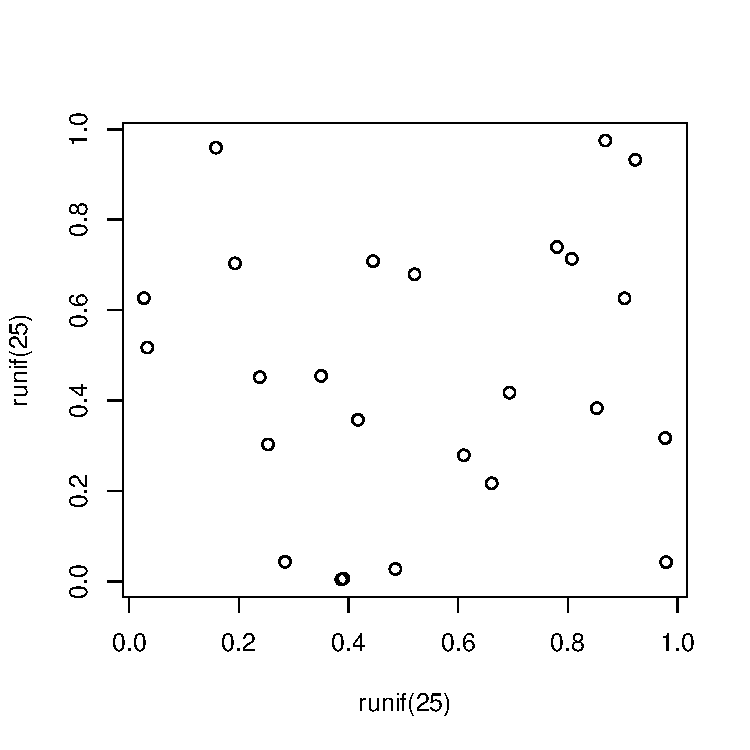
\includegraphics[width=0.5\linewidth]{ArtigoElsevier_files/figure-latex/fig2-1} 

}

\caption{\label{fig2}A meaningless scatterplot.}\label{fig:fig2}
\end{figure}

\section{Tables coming from R}\label{tables-coming-from-r}

Tables can also be generated using R chunks, as shown in Table
\ref{tab1} for example.

\begin{Shaded}
\begin{Highlighting}[]
\NormalTok{knitr}\SpecialCharTok{::}\FunctionTok{kable}\NormalTok{(}\FunctionTok{head}\NormalTok{(mtcars)[,}\DecValTok{1}\SpecialCharTok{:}\DecValTok{4}\NormalTok{], }
    \AttributeTok{caption =} \StringTok{"}\SpecialCharTok{\textbackslash{}\textbackslash{}}\StringTok{label\{tab1\}Caption centered above table"}
\NormalTok{)}
\end{Highlighting}
\end{Shaded}

\begin{longtable}[]{@{}lrrrr@{}}
\caption{\label{tab1}Caption centered above table}\tabularnewline
\toprule\noalign{}
& mpg & cyl & disp & hp \\
\midrule\noalign{}
\endfirsthead
\toprule\noalign{}
& mpg & cyl & disp & hp \\
\midrule\noalign{}
\endhead
\bottomrule\noalign{}
\endlastfoot
Mazda RX4 & 21.0 & 6 & 160 & 110 \\
Mazda RX4 Wag & 21.0 & 6 & 160 & 110 \\
Datsun 710 & 22.8 & 4 & 108 & 93 \\
Hornet 4 Drive & 21.4 & 6 & 258 & 110 \\
Hornet Sportabout & 18.7 & 8 & 360 & 175 \\
Valiant & 18.1 & 6 & 225 & 105 \\
\end{longtable}

\section*{References}\label{references}
\addcontentsline{toc}{section}{References}

\end{document}
